\section*{Задание 1: Секундомер с драйвером 4026}
\begin{verbatim}
          Последовательность: составных чисел (A002808)
          Сборка (общ.): счётчик нажатий.
\end{verbatim}
\noindent
\textbf{Код прошивки 1:}
\lstinputlisting{z1.cpp}
\noindent
\indent
Код реализует счётчик нажатий,
отображающий на семисегментных индикаторах (с драйвером 4026) последовательность составных чисел.
При каждом нажатии кнопки инкрементируется счётчик,
и на индикатор выводится очередное составное число.
При достижении предела (например, 99) счётчик сбрасывается.
\newpage
\section*{Задание 2: Счётчик нажатий/секундомер на ЗЛС338А}
\begin{verbatim}
          Последовательность: Двоичные палиндромы (A006995)
          Сборка (общ.): счётчик нажатий.
\end{verbatim}
\noindent
\textbf{Код прошивки 2:}
\lstinputlisting{z2.cpp}
\noindent
\indent
Программа управляет двуразрядным семисегментным индикатором методом динамической индикации.
\newpage
\section*{Задание 3: Секундомер на микросхеме К176ИЕ4}
\begin{verbatim}
          Последовательность: числа Харшад (A005349)
          Сборка (общ.): катод.
\end{verbatim}
% Сборка в живую.
\noindent
\textbf{Код прошивки 3:}
\lstinputlisting{z3.cpp}
\noindent
\indent
Микросхема К176ИЕ4 используется как двоично-десятичный счётчик.
Микроконтроллер формирует последовательность чисел Харшад и подаёт их на счётчик,
который управляет семисегментным индикатором.
Перебор чисел происходит автоматически с заданной задержкой.
\newpage
\section*{Задание 4: Вывод текста}
\begin{verbatim}
          ЖК экран: без I2C
          Навигация: потенциометр
          Управление подсветкой: кнопки
\end{verbatim}
\begin{figure}[H]
	\centering
	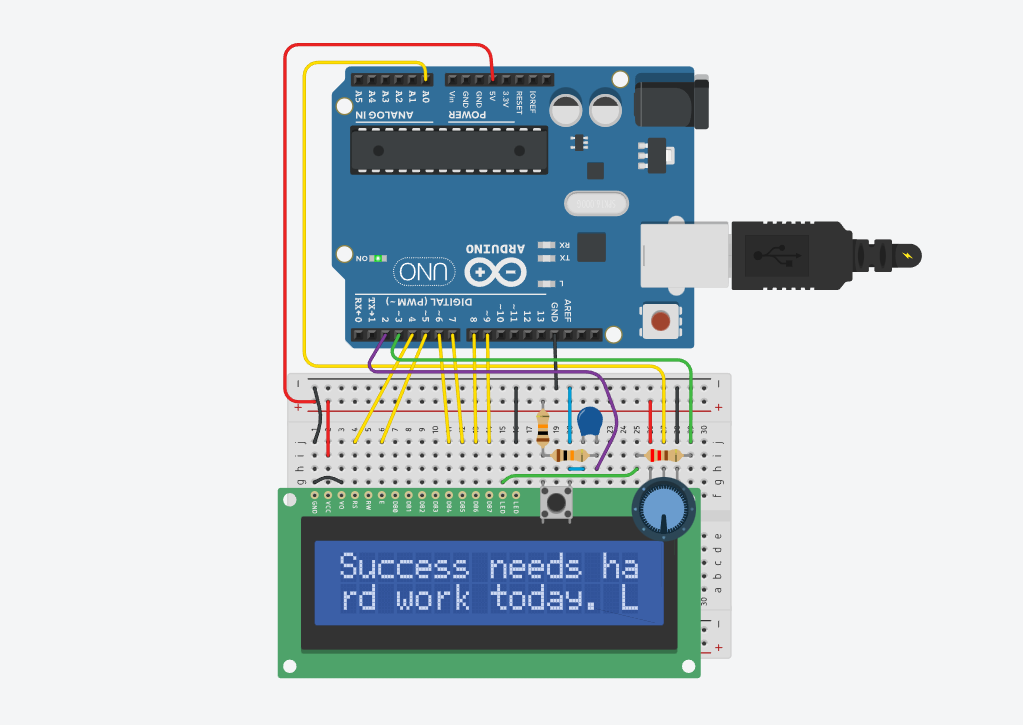
\includegraphics[width=17cm]{z4/1.png}
	\caption{схема сборки}
\end{figure}
\begin{figure}[H]
	\centering
	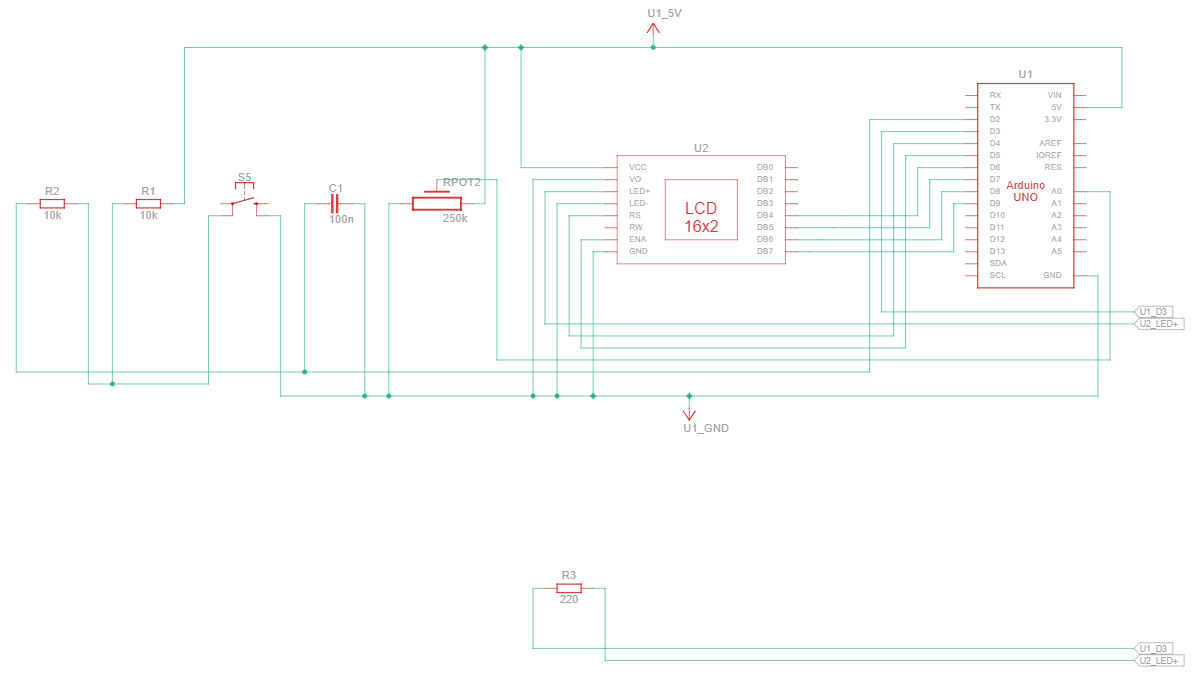
\includegraphics[width=17cm]{z4/2.png}
	\caption{принципиальная схема}
\end{figure}
\noindent
\textbf{Код прошивки 4:}
\lstinputlisting{z4/code.cpp}
\noindent
\indent
Программа выводит на символьный ЖК-дисплей 16x2 заданный текст.
Потенциометр прокручивает текст вверх/вниз, кнопки включают/выключают подсветку.
\newline
\noindent
\textbf{Ссылка на рабочий проект:}
\href{https://www.tinkercad.com/things/d9Z8SE4pRKq-l2z4?sharecode=h3XRbBuXqSVTGQkRF7nr2eDlebL4yIaNlWw6IdcImpQ}{Tinkercad}

% \section*{Задание 5: Задание с мотором}
% Вариант 5: \textbf{не выполнено}. Задание находится в стадии разработки.

\newpage
\section*{Задание 6: Светодиодная матрица 8x8 (Toyka модуль)}
Отобразить три состояния (анимация):
\begin{figure}[H]
	\centering
	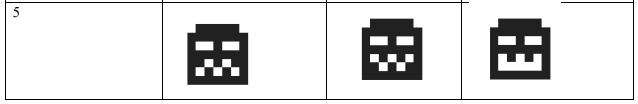
\includegraphics[width=17cm]{6.png}
	\caption{исходные изображения}
\end{figure}
\noindent
\textbf{Код прошивки 6:}
\lstinputlisting{z6.cpp}
\noindent
\indent
На матрице 8x8 последовательно выводятся три графических состояния.
Переход между состояниями осуществляется по таймеру.
\newpage
\section*{Задание 7: Светодиодная матрица АЛС340А1}
Вывести первую букву фамилии и затем номер варианта (5) поочерёдно.
\noindent
\textbf{Код прошивки 7:}
\lstinputlisting{z7.cpp}
\noindent
\indent
Программа формирует на матрице АЛС340А1 (8x8) изображение первой буквы фамилии студента (например, «Г»), затем через секунду — цифру «5». Цикл повторяется. Используется динамическая индикация для управления отдельными светодиодами.